\documentclass[12pt,a4paper,titlepage]{article}
\usepackage[utf8]{inputenc}
\usepackage{polski}
\usepackage{listings}
\usepackage{natbib}
\usepackage{graphicx}
\usepackage{xcolor}
\usepackage{listings}
\usepackage{minted}
\usepackage{amsmath,latexsym}
\usepackage{caption}
\usepackage{float}
\usepackage{graphicx}
\usepackage{tikz}
\usepackage{pgfplots}
\usepackage{pgfgantt}
\usepackage{algpseudocode}
\usepackage{algorithm}
\usepackage{longtable}


\usepackage[colorlinks = true,
            linkcolor = black,
            urlcolor  = blue,
            citecolor = blue,
            anchorcolor = blue]{hyperref}

\pgfplotsset{compat=1.15} 

\DeclareCaptionType{myequation}[][Równanie parametryczne]
\captionsetup[myequation]{labelformat=empty}

\makeatletter
\newcommand{\linia}{\rule{\linewidth}{0.4mm}}
\renewcommand{\maketitle}{\begin{titlepage}
    \vspace*{1cm}
    \begin{center}\small
    Politechnika Wrocławska\\
    Wydział Elektroniki\\
    Programowanie Efektywnych Algorytmów
    \end{center}
    \vspace{3cm}
    \noindent\linia
    \begin{center}
      \LARGE \textsc{\@title}
         \end{center}
     \linia
    \vspace{0.5cm}
    \begin{flushright}
    \begin{minipage}{7cm}
    \textit{\small Autor:}\\
    \normalsize \textsc{\@author} \par
    \end{minipage}
    \vspace{5cm}

     {\small Poniedziałek, 11\textsuperscript{15}-13\textsuperscript{00}}\\
        Dr inż. Jarosław Rudy
     \end{flushright}
    \vspace*{\stretch{6}}
    \begin{center}
    \@date
    \end{center}
  \end{titlepage}
}
\makeatother
\author{Justyna Skalska, 225942}
\title{Problem Komiwojażera\\
\large{(Algorytm genetyczny \& Algorytm mrówkowy)}}

\begin{document}
\maketitle
\tableofcontents

\newpage

\section{Wstęp}
\subsection{Cel projektu}
Celem projektu było wykonanie programu wykorzystującego algorytm genetyczny (Genetic Algorithm) oraz algorytmu mrówkowego (Ant Optimization Algorithm) do rozwiązania problemu komiwojażera (Travelling Salesman Problem).

\subsection{Opis problemu}
Problem komiwojażera należy do klasy problemów NP-trudnych i jest on zagadnieniem optymalizacyjnym, polegającym na znalezieniu minimalnego cyklu Hamiltona w pełnym grafie ważonym. Mówiąc prościej, rozwiązaniem problemu komiwojażera jest znalezienie najkrótszej ścieżki w grafie skierowanym, rozpoczynającej się w danym wierzchołku, odwiedzającej wszystkie wierzchołki dokładnie raz i kończącej się w wierzchołku początkowym. Ścieżka taka nazywa się optymalną trasą. Ponieważ nie ma znaczenia, gdzie zaczynamy, wierzchołek początkowy może być po prostu pierwszym wierzchołkiem w grafie. W wersji asynchronicznej, odległości pomiędzy wierzchołkami mogą dodatkowo zależeć także od kierunku przejścia pomiędzy nimi. Główną trudnością w rozwiązaniu problemu jest znacząca liczba możliwych kombinacji.

\subsection{Opis instancji}
Podczas testów wykorzystane zostały instancje zamieszczone na stronie \newline \href{https://www.iwr.uni-heidelberg.de/groups/comopt/software/TSPLIB95/}{TSPLIB}. Dane w nagłówku plików zapisane są za pomocą klucza i wartości. Najważniejsze w tym przypadku są "EDGE\_WEIGHT\_TYPE" oraz "EDGE\_WEIGHT\_FORMAT", dzięki którym wiemy w jakim formacie graf został zapisany w pliku. Sczytujemy liczbę wierzchołków używając klucza "DIMENSION", a dane o grafie pobieramy z sekcji znajdującej się pod "EDGE\_WEIGHT\_SECTION". Do pomiarów wykorzystano także instancje testowe ze \href{http://jaroslaw.mierzwa.staff.iiar.pwr.wroc.pl/pea-stud/tsp/}{strony doktora Jarosława Mierzwy}, które pozwalają zmierzyć czas wykonywania algorytmu dla liczby wierzchołków wykorzystanej przy testach poprzednio zaimplementowanych algorytmów. Dzięki temu mogę porównać ich działanie. Każdy z tych plików zawiera liczbę wierzchołków grafu zamieszczoną w pierwszej linii oraz ich wagi przedstawione w postaci macierzy sąsiedztwa.

\subsection{Specyfikacja techniczna}
\subsubsection{Opis sprzętu}
\begin{itemize}
    \item System operacyjny: MacOS Mojave - wersja 10.14.1 (18B75),
    \item Procesor: 2,2 GHz Intel Core i7-4770HQ,
    \item Pamięć: 16 GB 1600 MHz DDR3,
    \item IDE: CLion 2018.2.5
\end{itemize}
\subsubsection{Opis programu}
\begin{itemize}
    \item Program został wykonany obiektowo w języku C++,
    \item Program akceptuje dane wczytywane z pliku, dla symetrycznego oraz asymetrycznego problemu komiwojażera,
    \item Czas wykonania algorytmów mierzony był przy wykorzystaniu biblioteki std::chrono,
    \item Do dynamicznego przechowywania danych została wykorzystana biblioteka std::vector.
\end{itemize}

\section{Opis algorytmów}
\subsection{Wstęp teoretyczny}
\subsubsection{Opis teoretyczny}
Heurystyka jest techniką, która znajduje dobre rozwiązania przy akceptowalnych nakładach obliczeniowych, ale bez gwarancji osiągalności czy optymalności celu, czy nawet - w  wielu przypadkach – jak blisko optymalnego jest otrzymane rozwiązanie.\cite{agh}
\\\\
Metaheurystyka - ogólny algorytm (heurystyka) do rozwiązywania problemów obliczeniowych. Algorytm metaheurystyczny można używać do rozwiązywania dowolnego problemu, który można opisać za pomocą pewnych definiowanych przez ten algorytm pojęć. Algorytmy tego typu nie służą do rozwiązywania konkretnych problemów, a jedynie podają sposób na utworzenie odpowiedniego algorytmu.\cite{agh}

\subsection{Algorytm genetyczny}
\subsubsection{Opis teoretyczny}
Algorytm genetyczny to metaheurystyka inspirowana procesem doboru naturalnego, który należy do klasy algorytmów ewolucyjnych. Algorytmy genetyczne są powszechnie używane do generowania wysokiej jakości rozwiązań w zakresie optymalizacji i wyszukiwania problemów, polegając na inspirowanych biologią operatorach, takich jak mutacja, crossover i selekcja. John Holland wprowadził algorytmy genetyczne w 1960 roku w oparciu o koncepcję teorii ewolucji Darwina, a później jego student Goldberg rozszerzył GA w 1989 roku.\cite{wiki_ga}\\\\
Algorytm genetyczny wykorzystuje techniki inspirowane biologią ewolucyjną, takie jak selekcja, mutacja, dziedziczenie i rekombinacja, aby rozwiązać problem. Najczęściej stosowaną metodą w algorytmach genetycznych jest tworzenie grupy osobników losowo wybranych z danej populacji. Tak utworzone jednostki są oceniane za pomocą funkcji oceny, która pośrednio określa przydatność (ang. fitness) do danej sytuacji.
Najlepsze dwa osobniki są następnie używane do stworzenia jednego lub więcej potomstwa. Następnie wykonywane wykonywane są losowe mutacje na potomkach.\\\\
Algorytm genetyczny różni się od poprzednio zaimplementowanych algorytmów, ponieważ generuje populację on punktów w każdej iteracji, podczas gdy poprzednie algorytmy generują pojedynczy punkt w każdej iteracji. Algorytm genetyczny wybiera następną populację przez obliczenia za pomocą generatorów liczb losowych, podczas gdy klasyczne algorytmy wybierają następny punkt za pomocą deterministycznego obliczania.

\paragraph{Crossover}\mbox{}\\
Crossover, zwany także rekombinacją, jest stosowany do łączenia informacji genetycznej dwóch rodziców w celu wygenerowania nowego potomstwa. Jest wiele typów rekombinacji, a dwa z nich zostały wykorzystane w projekcie:

\begin{itemize}
    \item Multi point crossover z inwersją \\\\
    Na początku wybierane są dwa losowe punkty, które tworzą podciągi w obu rodzicach. Środkowe podciągi są odwracane (ostatni element zamieniany z pierwszym itd.), a następnie umieszczane w potomkach. Geny z pierwszego rodzica przechodzą do drugiego dziecka i na odwrót. Następnie uzupełnia się dziecko pierwsze o brakujące elementy z rodzina pierwszego. To samo wykonuje się dla drugiego potomka.
    \begin{figure}[H]
    \centering
    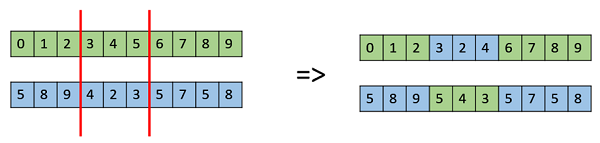
\includegraphics[width = 14cm]{images/multi_point_crossover.png}
    \caption{Multi point crossover z inwersją \cite{ga_crossover}}
    \label{fig:mpxi}
    \end{figure}
    \item Order crossover (OX) \\\\
    Algorytm ten jest używany do crossoverów opartych na permutacjach, gdzie ważne jest zachowanie informacji o kolejności genów rodzica przenoszonych do potomka. Na początku wybierane są dwa losowe punkty, które tworzą podciągi w obu rodzicach. Środkowy podciąg z pierwszego rodzica przekazywany jest pierwszemu potomkowi. Następnie zaczynając od drugiego wylosowanego wcześniej punktu w drugim rodzicu należy skopiować pozostałe, nieużywane geny do pierwszego dziecka. Gdy przejdziemy do końca listy należy przejść do jej początku i kontynuować kopiowanie. Ostatnim krokiem jest powtórzenie algorytmu dla drugiego dziecka.
    \begin{figure}[H]
    \centering
    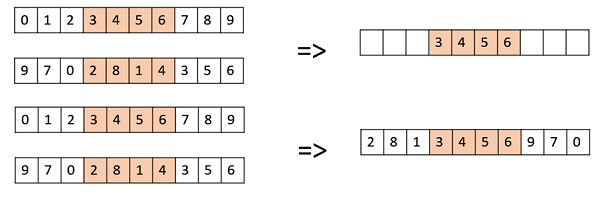
\includegraphics[width = 14cm]{images/david_order_crossover.jpg}
    \caption{Order crossover (OX) \cite{ga_crossover}}
    \label{fig:ox}
    \end{figure}
\end{itemize}

\paragraph{Mutacja}\mbox{}\\
Mutacja jest stosowana w celu utrzymania i wprowadzenia różnorodności w populacji genetycznej. Jest zwykle stosowana z małym prawdopodobieństwem.. Jeśli prawdopodobieństwo jest bardzo wysokie, GA zostaje zredukowane do losowego wyszukiwania. Mutacja jest częścią GA związaną z "eksploracją" przestrzeni poszukiwań. Zaobserwowano, że mutacja jest niezbędna do zbieżności GA, podczas gdy krzyżowanie nie jest. Jest wiele typów mutacji, a dwa z nich zostały wykorzystane w projekcie:
\begin{itemize}
    \item Mutacja swap \\\\
    W tego typie mutacji wybieramy losowo dwie pozycje na chromosomie i wymieniamy wartości. Jest to powszechne w kodowaniach opartych na permutacji.
    \begin{figure}[H]
    \centering
    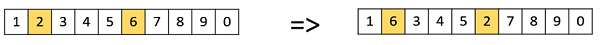
\includegraphics[width = 14cm]{images/swap_mutation.jpg}
    \caption{Mutacja swap \cite{ga_mutation}}
    \label{fig:swap}
    \end{figure}
    \item Mutacja scramble \\\\
    Mutacja ta jest również popularna w reprezentacjach opartych na permutacjach. W tym przypadku z całego chromosomu wybiera się podzbiór genów, a ich wartości są losowo mieszane lub losowane.
    \begin{figure}[H]
    \centering
    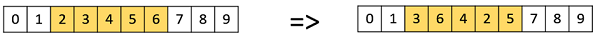
\includegraphics[width = 14cm]{images/scramble_mutation.jpg}
    \caption{Mutacja scramble \cite{ga_mutation}}
    \label{fig:scramble}
    \end{figure}
\end{itemize}

\subsubsection{Złożoność obliczeniowa}
Dla algorytmu genetycznego nie byłam w stanie znaleźć teoretycznej złożoności obliczeniowej. Udało mi się dowiedzieć, że jest ona podobna do złożoności zaimplementowanego algorytmu mrówkowego.

\subsubsection{Pseudokod}
\begin{algorithm}[H]
\caption{Pseudokod dla algorytmu genetycznego}
\begin{algorithmic}
\Require $generations$
\State $realPopulationSize \gets initializePopulation()$
\If{$realPopulationSize == 0$}
    \State \Return $0$
\EndIf
\State $sortPopulation()$
\For{$i \gets 0$ \textbf{to} $generations$}
    \State $oldPopulationSize \gets realPopulationSize$
    \State $crossover()$
    \State $mutation()$
    \State $updatePopulation(oldPopulationSize)$
\EndFor
\State \Return $best$
\end{algorithmic}
\end{algorithm}

Mutacja jest stosowana do utrzymania różnorodności genetycznej z jednego pokolenia populacji chromosomów algorytmu genetycznego do następnego. Jest to analogiczne do mutacji biologicznej

\subsubsection{Opis implementacji}
Pierwszym krokiem algorytmu jest inicjalizacja populacji poprzez generowanie losowych permutacji dla początkowego ciągu. Jeśli sekwencja jest poprawna, czyli istnieje taka ścieżka, to jest ona dodawana do populacji i prawdziwy rozmiar populacji jest zwiększany o 1. Prawdziwy rozmiar populacji jest wykorzystywany w programie do aktualizacji populacji, gdy staje się ona większa niż początkowa. Następnym krokiem jest sprawdzenie czy populacja nie jest pusta. Jeśli tak program kończy swoje działanie. W przeciwnym wypadku populacja jest sortowana według wartości ścieżki.

\begin{listing}[H]
\caption{Struktura wykorzystywana przy sortowaniu elementów populacji}
\begin{minted}[autogobble,linenos,breaklines,frame=lines,framerule=0.5pt,framesep=10pt]{C++}
typedef std::pair<std::vector<int>, int> populationPair;

struct sortPopulation
{
    bool operator()(const populationPair& firstElem, const populationPair& secondElem)
    {
        return firstElem.second < secondElem.second;
    }
};
\end{minted}
\end{listing}
Kolejnym etapem jest pętla, której warunkiem końca jest określona z góry liczba generacji. W jej wnętrzu wykonywane jest krzyżowanie, mutacja oraz aktualizacja populacji. Rodzice do krzyżowania wybierani są losowo i muszą się od siebie różnić. Następnie wybierana jest metoda krzyżowania OX lub MPXI. Po jej wykonaniu następuje mutacja, która może wykonać się lub nie zależnie od wylosowanego prawdopodobieństwa. Później wybierana jest metoda mutacji poprzez zamianę lub mieszanie. Ostatnim krokiem pętli jest aktualizacja populacji, czyli sprawdzenie czy została ona zwiększona, jeśli tak to najgorsze osobniki zostaną z niej usunięte. Po skończeniu pętli najlepszy uzyskany wynik zostaje zwrócony.

\subsection{Algorytm mrówkowy}
\subsubsection{Opis teoretyczny}
Algorytm mrówkowy jest probabilistyczną techniką rozwiązywania problemów obliczeniowych, które można zredukować do znalezienia najlepszych ścieżek w grafie. Metoda ta po raz pierwszy została opisana przez Marco Dorigo w jego pracy doktorskiej. Nawiązuje ona do świata mrówek i sposobu w jaki wybierają one drogę od mrowiska do pożywienia. Na początku mrówki wybierają ścieżkę losowo pozostawiając za sobą feromony, które parują z określoną prędkością. Jeśli kolejna mrówka wybierze tę samą trasę to wzmocni ona ślad feromonów. Im krótsza trasa tym wolniej one parują. Im mocniejszy ślad feromonów tym chętniej trasa będzie wybierana przez mrówki, które za każdym przejściem będą wzmacniać ślad.
\\\\
Na początku generowana jest populacja mrówek, która jest jednym z parametrów algorytmu. Każdy z osobników generuje swoją ścieżkę niezależnie od reszty, a miasto początkowe jest generowane losowo. Posiadają one także listę już odwiedzonych wierzchołków, aby zapobiec wracaniu do poprzednich punktów. Mrówki poruszają się po grafie w poszukiwaniu najkrótszej ścieżki zostawiając na swojej trasie feromony, które mają wpływ na wybór ścieżki przez kolejne osobniki. Każdy następny wybrany przez mrówkę wierzchołek jest losowy, ale na wybór ma wpływ także ilość feromonu oraz długość ścieżki.
\\\\
Prawdopodobieństwo przejścia $k$-tej mrówki ze stanu $x$ do stanu $z$ określone jest wzorem:
\begin{myequation}[H]
\begin{equation}
    \begin{split}
    &p^{k}_{xy} = \dfrac{(\tau^{\alpha}_{xy})(\eta^{\beta}_{xy})}{\Sigma_{z\in dozwolone_{x}}(\tau^{\alpha}_{xz})(\eta^{\beta}_{xz})} \\\\
    &\tau^{\alpha}_{xy} - \text{ilość feromonu pozostawiona przy przejściu z $x$ do $y$} \\
    &\eta^{\beta}_{xy} - \text{atrakcyjność przejścia z $x$ do $y$} \\
    &\tau^{\alpha}_{xz} \text{ oraz } \eta^{\beta}_{xz} - \text{reprezentują atrakcyjność i poziom szlaku} \\
    &\text{dla pozostałych przejść} \\
    &\alpha - \text{określa jaki wpływ na prawdopodobieństwo ma }\tau^{\alpha}_{xy} \\
    &\beta - \text{określa jaki wpływ na prawdopodobieństwo ma }\eta^{\beta}_{xy}
    \end{split}
\end{equation}
\caption{Prawdopodobieństwo przejścia $k$-tej mrówki ze stanu $x$ do stanu $z$}
\end{myequation}
Po przejściu drogi przez wszystkie mrówki w danej iteracji wyznacza się nowe punkty początkowe skąd owady rozpoczną swoją trasę, a feromony przez nie pozostawione są aktualizowane. W miarę upływu czasu zmniejszają one swoją ilość.
\begin{myequation}[H]
\begin{equation}
    \begin{split}
        &\tau_{xy}\gets(1- \rho)\tau_{xy} + \sum\limits_{k}\Delta\tau^{k}_{xy} \\\\
        \Delta\tau^{k}_{xy} = 
        &\begin{cases}
            \dfrac{Q}{L_{k}} & \text{jeśli mrówka $k$ przechodzi przez ścieżkę $xy$} \\
            0 & \text{w przeciwnym wypadku}
        \end{cases} \\\\
        &\tau_{xy} - \text{ilość pozostawionego feromonu przez $k$-tą mrówkę} \\
        &\rho - \text{współczynnika parowania feromonów} \\
        &\text{przy przejściu z $x$ do $y$} \\
        &L_{k} - \text{wartość ścieżki $k$-tej mrówki} \\
        &Q - \text{stała}
    \end{split}
\end{equation}
\caption{Aktualizacja ścieżek}
\end{myequation}

\subsubsection{Złożoność obliczeniowa}
Złożoność algorytmu mrówkowego wynosi\cite{aco_pwr}:
\begin{myequation}[H]
\begin{equation}
    \begin{split}
        &O(C*n^{2}*m) \\
        &C - \text{liczba iteracji (cykli)}
    \end{split}
\end{equation}
\end{myequation}

\begin{flushleft}
Dorigo i jego ludzie znaleźli liniową zależność pomiędzy liczbą mrówek a liczbą miast.
Stąd można przyjąć, że złożoność obliczeniowa dla $m = n$ wynosi:
\end{flushleft}

\begin{myequation}[H]
\begin{equation}
    \begin{split}
        &O(C*n^{3}) \\
        &C - \text{liczba iteracji (cykli)}
    \end{split}
\end{equation}
\end{myequation}

\subsubsection{Pseudokod}
\begin{algorithm}[H]
\caption{Pseudokod dla algorytmu mrówkowego}
\begin{algorithmic}
\Require $maxTours$
\State $currentIteration \gets 0$
\State $maxIterations \gets maxTours * numberOfVertexes$
\State $initialize()$
\While{$currentIteration++ < maxIterations$}
    \If{$availableVertexes != 0$}
        \State $best \gets simulateAnts()$
        \State $updateTrials()$
        \If{$currentIteration != maxIterations$}
            \State $restartAnts()$
        \EndIf
    \EndIf
\EndWhile
\State \Return $best$
\end{algorithmic}
\end{algorithm}

\subsubsection{Opis implementacji}
Pierwszym krokiem jest zainicjalizowanie feromonów dla poszczególnych wierzchołków oraz populacji mrówek. Następnie wykonywana jest pętla, której liczba iteracji odpowiada parametrowi maksymalnej liczby "wycieczek" pomnożonemu przez liczbę wierzchołków grafu. Kolejnym krokiem jest wybranie ścieżki jaką przemieści się każda z mrówek. Mrówki mają zaimplementowaną listę tabu punktów, które odwiedziły w przeszłości, więc nie mogą przejść do miejsca w którym już wcześniej były. Po przejściu mrówek przez wybrane ścieżki następuje aktualizacja wartości feromonów poszczególnych ścieżek. Jeśli nie jest to ostatnia iteracja pętli to ścieżka oraz lista tabu osobników są reinicjalizowane, a najlepsza znaleziona wartość ścieżki jest zapisywana do zmiennej, jeśli jest ona mniejsza niż poprzednia.

\section{Pomiary}
Test zostanie wykonany dla 5 symetrycznych oraz 2 asymetrycznych instancjach problemu komiwojażera, dla których rozwiązanie optymalne jest znane. Dla każdej instancji problemu oraz zestawienia algorytmu z jego parametrami zostanie wykonane 10 pomiarów, które zostaną później uśrednione.
\newpage
\begin{flushleft}
Instancje dla symetrycznego problemu komiwojażera:
\end{flushleft}
\begin{itemize}
    \item Nazwa instancji: 10.txt
    \begin{itemize}
        \item Rozmiar: 10
        \item Rozwiązanie optymalne: 212
    \end{itemize}
    \item Nazwa instancji: 15.txt
    \begin{itemize}
        \item Rozmiar: 15
        \item Rozwiązanie optymalne: 291
    \end{itemize}
    \item Nazwa instancji: gr21.tsp
    \begin{itemize}
        \item Rozmiar: 21
        \item Rozwiązanie optymalne: 2707
    \end{itemize}
    \item Nazwa instancji: gr48.tsp
    \begin{itemize}
        \item Rozmiar: 48
        \item Rozwiązanie optymalne: 5046
    \end{itemize}
    \item Nazwa instancji: gr120.tsp
    \begin{itemize}
        \item Rozmiar: 120
        \item Rozwiązanie optymalne: 6942
    \end{itemize}
\end{itemize}
\vspace{1cm}
Instancje dla niesymetrycznego problemu komiwojażera:

\begin{itemize}
    \item Nazwa instancji: ftv47.atsp
    \begin{itemize}
        \item Rozmiar: 47
        \item Rozwiązanie optymalne: 1776
    \end{itemize}
    \item Nazwa instancji: ftv170.atsp
    \begin{itemize}
        \item Rozmiar: 170
        \item Rozwiązanie optymalne: 2755
    \end{itemize}
%    \item Nazwa instancji: rgb403.atsp
%    \begin{itemize}
%        \item Rozmiar: 403
%        \item Rozwiązanie optymalne: 2465
%    \end{itemize}
\end{itemize}

\subsection{Algorytm genetyczny}
Algorytm został przetestowany dla populacji wynoszącej: 10, 50, 80, 150. Prawdopodobieństwo krzyżowania wynosiło: 0.9, 0.5, 0.4, a prawdopodobieństwo mutacji: 0.1, 0.2, 0.3, 0.5. Liczba iteracji równała się: 100, 1000, 10000.
Przy testowaniu wszystkich wariantów algorytmu powstało wiele wyników, wobec czego tylko część została zamieszczona w sprawozdaniu. Przedstawiłam tutaj tylko najlepsze wyniki dla algorytmu genetycznego.
\begin{table}[H]
	\caption{Najlepsze wyniki otrzymane dla algorytmu genetycznego}
    \centering
	\begin{tabular}{|p{0.14\linewidth}|p{0.09\linewidth}|p{0.12\linewidth}|p{0.15\linewidth}|p{0.1\linewidth}|p{0.15\linewidth}|p{0.06\linewidth}|p{0.06\linewidth}|}
		\hline
        Instancji & Liczba\newline iteracji & Rozmiar populacji & Prawd. krzyżowania & Prawd. mutacji & Otrzymane rozwiązanie & Błąd & Czas (ms) \\
		\hline
        10.txt & 100 & 10 & 0.9 & 0.1 & 212 & 0\% & 140 \\
        \hline
        15.txt & 100 & 10 & 0.9 & 0.1 & 291 & 0\% & 185 \\
        \hline
        gr21.tsp & 1000 & 10 & 0.9 & 0.1 & 2707 & 0\% & 289 \\
        \hline
        gr48.tsp & 10000 & 50 & 0.9 & 0.2 & 5046 & 0\% & 1010 \\
        \hline
        gr120.tsp & 10000 & 50 & 0.5 & 0.2 & 7121 & 3\% & 3027 \\
        \hline
        ftv47.atsp & 10000 & 80 & 0.5 & 0.2 & 1902 & 7\% & 641 \\
        \hline
        ftv170.atsp & 10000 & 80 & 0.5 & 0.3 & 3251 & 18\% & 3847 \\
        \hline
    \end{tabular}
\end{table}

\subsection{Algorytm mrówkowy}
Algorytm został przetestowany dla populacji mrówek wynoszącej: 10, 20, 50, 100, 150. Tempo parowania wynosiło: 0.02, 0.2, 0.4, 0.6, 0.8. Maksymalna liczba "wycieczek" (ang. tours) wynosiła: 10, 20, 50, 100, 150.
\\\\
W tabelach przedstawiono wyniki tylko dla populacji mrówek zbliżonej do ilości miast. Dawała ona najlepsze wyniki dla większych instancji względem pozostałych populacji. Warto tu zwrócić uwagę na zależność jaką znaleźli Dorigo i jego ludzie, czyli liniową zależność pomiędzy liczbą mrówek a liczbą miast.

\begin{table}[H]
	\caption{Algorytm mrówkowy dla instancji 10.txt}
    \centering
	\begin{tabular}{|p{0.15\linewidth}|p{0.10\linewidth}|p{0.16\linewidth}|p{0.18\linewidth}|p{0.07\linewidth}|p{0.17\linewidth}|}
		\hline
        Populacja mrówek & Tempo parowania & Maksymalna liczba \newline wycieczek & Otrzymane rozwiązanie & Błąd & Czas \newline wykonywania (ms) \\
		\hline
		10 & 0.02 & 10 & 212 & 0\% & 0 \\
        10 & 0.02 & 20 & 212 & 0\% & 1 \\
        10 & 0.02 & 50 & 212 & 0\% & 4 \\
        10 & 0.02 & 100 & 212 & 0\% & 9 \\
        10 & 0.02 & 150 & 212 & 0\% & 13 \\
        \hline
        10 & 0.2 & 10 & 212 & 0\% & 0 \\
        10 & 0.2 & 20 & 212 & 0\% & 1 \\
        10 & 0.2 & 50 & 212 & 0\% & 4 \\
        10 & 0.2 & 100 & 212 & 0\% & 9 \\
        10 & 0.2 & 150 & 212 & 0\% & 13 \\
        \hline
        10 & 0.4 & 10 & 212 & 0\% & 0 \\
        10 & 0.4 & 20 & 212 & 0\% & 1 \\
        10 & 0.4 & 50 & 212 & 0\% & 4 \\
        10 & 0.4 & 100 & 212 & 0\% & 8 \\
        10 & 0.4 & 150 & 212 & 0\% & 12 \\
        \hline
        10 & 0.6 & 10 & 212 & 0\% & 0 \\
        10 & 0.6 & 20 & 212 & 0\% & 1 \\
        10 & 0.6 & 50 & 212 & 0\% & 4 \\
        10 & 0.6 & 100 & 212 & 0\% & 8 \\
        10 & 0.6 & 150 & 212 & 0\% & 12 \\
        \hline
        10 & 0.8 & 10 & 212 & 0\% & 0 \\
        10 & 0.8 & 20 & 212 & 0\% & 1 \\
        10 & 0.8 & 50 & 212 & 0\% & 4 \\
        10 & 0.8 & 100 & 212 & 0\% & 8 \\
        10 & 0.8 & 150 & 212 & 0\% & 13 \\
        \hline
    \end{tabular}
\end{table}

\begin{table}[H]
	\caption{Algorytm mrówkowy dla instancji 15.txt}
    \centering
	\begin{tabular}{|p{0.15\linewidth}|p{0.10\linewidth}|p{0.16\linewidth}|p{0.18\linewidth}|p{0.07\linewidth}|p{0.17\linewidth}|}
		\hline
        Populacja mrówek & Tempo parowania & Maksymalna liczba \newline wycieczek & Otrzymane rozwiązanie & Błąd & Czas \newline wykonywania (ms) \\
		\hline
        20 & 0.02 & 10 & 291 & 0\% & 3 \\
        20 & 0.02 & 20 & 291 & 0\% & 7 \\
        20 & 0.02 & 50 & 291 & 0\% & 18 \\
        20 & 0.02 & 100 & 291 & 0\% & 37 \\
        20 & 0.02 & 150 & 291 & 0\% & 55 \\
        \hline
        20 & 0.2 & 10 & 291 & 0\% & 3 \\
        20 & 0.2 & 20 & 291 & 0\% & 7 \\
        20 & 0.2 & 50 & 291 & 0\% & 19 \\
        20 & 0.2 & 100 & 291 & 0\% & 37 \\
        20 & 0.2 & 150 & 291 & 0\% & 56 \\
        \hline
        20 & 0.4 & 10 & 291 & 0\% & 3 \\
        20 & 0.4 & 20 & 291 & 0\% & 7 \\
        20 & 0.4 & 50 & 291 & 0\% & 18 \\
        20 & 0.4 & 100 & 291 & 0\% & 37 \\
        20 & 0.4 & 150 & 291 & 0\% & 55 \\
        \hline
        20 & 0.6 & 10 & 291 & 0\% & 3 \\
        20 & 0.6 & 20 & 291 & 0\% & 7 \\
        20 & 0.6 & 50 & 291 & 0\% & 18 \\
        20 & 0.6 & 100 & 291 & 0\% & 39 \\
        20 & 0.6 & 150 & 291 & 0\% & 56 \\
        \hline
        20 & 0.8 & 10 & 291 & 0\% & 3 \\
        20 & 0.8 & 20 & 291 & 0\% & 7 \\
        20 & 0.8 & 50 & 291 & 0\% & 18 \\
        20 & 0.8 & 100 & 291 & 0\% & 38 \\
        20 & 0.8 & 150 & 291 & 0\% & 56 \\
        \hline
    \end{tabular}
\end{table}

\begin{table}[H]
	\caption{Algorytm mrówkowy dla instancji gr21.tsp}
    \centering
	\begin{tabular}{|p{0.15\linewidth}|p{0.10\linewidth}|p{0.16\linewidth}|p{0.18\linewidth}|p{0.07\linewidth}|p{0.17\linewidth}|}
		\hline
        Populacja mrówek & Tempo parowania & Maksymalna liczba \newline wycieczek & Otrzymane rozwiązanie & Błąd & Czas \newline wykonywania (ms) \\
		\hline
        20 & 0.02 & 10 & 2938 & 8\% & 6 \\
        20 & 0.02 & 20 & 2938 & 8\% & 13 \\
        20 & 0.02 & 50 & 2760 & 1\% & 34 \\
        20 & 0.02 & 100 & 2760 & 1\% & 69 \\
        20 & 0.02 & 150 & 2758 & 1\% & 106 \\
        \hline
        20 & 0.2 & 10 & 2938 & 8\% & 7 \\
        20 & 0.2 & 20 & 2938 & 8\% & 14 \\
        20 & 0.2 & 50 & 2760 & 1\% & 34 \\
        20 & 0.2 & 100 & 2760 & 1\% & 69 \\
        20 & 0.2 & 150 & 2758 & 1\% & 108 \\
        \hline
        20 & 0.4 & 10 & 2941 & 8\% & 7 \\
        20 & 0.4 & 20 & 2853 & 5\% & 13 \\
        20 & 0.4 & 50 & 2805 & 3\% & 35 \\
        20 & 0.4 & 100 & 2758 & 1\% & 69 \\
        20 & 0.4 & 150 & 2758 & 1\% & 106 \\
        \hline
        20 & 0.6 & 10 & 2941 & 8\% & 7 \\
        20 & 0.6 & 20 & 2853 & 5\% & 14 \\
        20 & 0.6 & 50 & 2805 & 3\% & 35 \\
        20 & 0.6 & 100 & 2758 & 1\% & 71 \\
        20 & 0.6 & 150 & 2758 & 1\% & 107 \\
        \hline
        20 & 0.8 & 10 & 2941 & 8\% & 7 \\
        20 & 0.8 & 20 & 2853 & 5\% & 13 \\
        20 & 0.8 & 50 & 2805 & 3\% & 34 \\
        20 & 0.8 & 100 & 2758 & 1\% & 69 \\
        20 & 0.8 & 150 & 2758 & 1\% & 106 \\
        \hline
    \end{tabular}
\end{table}

\begin{table}[H]
	\caption{Algorytm mrówkowy dla instancji gr48.tsp}
    \centering
	\begin{tabular}{|p{0.15\linewidth}|p{0.10\linewidth}|p{0.16\linewidth}|p{0.18\linewidth}|p{0.07\linewidth}|p{0.17\linewidth}|}
		\hline
        Populacja mrówek & Tempo parowania & Maksymalna liczba \newline wycieczek & Otrzymane rozwiązanie & Błąd & Czas \newline wykonywania (ms) \\
		\hline
        50 & 0.02 & 10 & 5726 & 13\% & 92 \\
        50 & 0.02 & 20 & 5726 & 13\% & 186 \\
        50 & 0.02 & 50 & 5726 & 13\% & 467 \\
        50 & 0.02 & 100 & 5701 & 12\% & 982 \\
        50 & 0.02 & 150 & 5597 & 10\% & 1489 \\
        \hline
        50 & 0.2 & 10 & 5762 & 14\% & 95 \\
        50 & 0.2 & 20 & 5264 & 4\% & 196 \\
        50 & 0.2 & 50 & 5264 & 4\% & 513 \\
        50 & 0.2 & 100 & 5264 & 4\% & 1017 \\
        50 & 0.2 & 150 & 5500 & 8\% & 1446 \\
        \hline
        50 & 0.4 & 10 & 5971 & 18\% & 94 \\
        50 & 0.4 & 20 & 5728 & 13\% & 184 \\
        50 & 0.4 & 50 & 5658 & 12\% & 466 \\
        50 & 0.4 & 100 & 5654 & 12\% & 930 \\
        50 & 0.4 & 150 & 5476 & 8\% & 1400 \\
        \hline
        50 & 0.6 & 10 & 5699 & 12\% & 93 \\
        50 & 0.6 & 20 & 5585 & 10\% & 189 \\
        50 & 0.6 & 50 & 5585 & 10\% & 466 \\
        50 & 0.6 & 100 & 5534 & 9\% & 932 \\
        50 & 0.6 & 150 & 5534 & 9\% & 1395 \\
        \hline
        50 & 0.8 & 10 & 5839 & 15\% & 94 \\
        50 & 0.8 & 20 & 5669 & 12\% & 189 \\
        50 & 0.8 & 50 & 5669 & 12\% & 461 \\
        50 & 0.8 & 100 & 5360 & 6\% & 925 \\
        50 & 0.8 & 150 & 5544 & 9\% & 1382 \\
        \hline
    \end{tabular}
\end{table}

\begin{table}[H]
	\caption{Algorytm mrówkowy dla instancji gr120.tsp}
    \centering
	\begin{tabular}{|p{0.15\linewidth}|p{0.10\linewidth}|p{0.16\linewidth}|p{0.18\linewidth}|p{0.07\linewidth}|p{0.17\linewidth}|}
		\hline
        Populacja mrówek & Tempo parowania & Maksymalna liczba \newline wycieczek & Otrzymane rozwiązanie & Błąd & Czas \newline wykonywania (ms) \\
		\hline
        100 & 0.02 & 10 & 8771 & 47\% & 1175 \\
        100 & 0.02 & 20 & 8757 & 47\% & 2340 \\
        100 & 0.02 & 50 & 8534 & 43\% & 5857 \\
        100 & 0.02 & 100 & 8536 & 43\% & 11819 \\
        100 & 0.02 & 150 & 8623 & 45\% & 17670 \\
        \hline
        100 & 0.2 & 10 & 8996 & 51\% & 1168 \\
        100 & 0.2 & 20 & 8675 & 45\% & 2347 \\
        100 & 0.2 & 50 & 8681 & 46\% & 5894 \\
        100 & 0.2 & 100 & 8531 & 43\% & 12144 \\
        100 & 0.2 & 150 & 8606 & 44\% & 18105 \\
        \hline
        100 & 0.4 & 10 & 8825 & 48\% & 1286 \\
        100 & 0.4 & 20 & 8439 & 42\% & 2457 \\
        100 & 0.4 & 50 & 8610 & 44\% & 6314 \\
        100 & 0.4 & 100 & 8491 & 42\% & 11957 \\
        100 & 0.4 & 150 & 8575 & 44\% & 18147 \\
        \hline
        100 & 0.6 & 10 & 8933 & 50\% & 1172 \\
        100 & 0.6 & 20 & 8612 & 44\% & 2348 \\
        100 & 0.6 & 50 & 8314 & 39\% & 5871 \\
        100 & 0.6 & 100 & 8420 & 41\% & 11704 \\
        100 & 0.6 & 150 & 8616 & 45\% & 17911 \\
        \hline
        100 & 0.8 & 10 & 8692 & 46\% & 1172 \\
        100 & 0.8 & 20 & 8805 & 48\% & 2364 \\
        100 & 0.8 & 50 & 8573 & 44\% & 6020 \\
        100 & 0.8 & 100 & 8562 & 44\% & 12295 \\
        100 & 0.8 & 150 & 8517 & 43\% & 18325 \\
        \hline
    \end{tabular}
\end{table}

\begin{table}[H]
	\caption{Algorytm mrówkowy dla instancji ftv47.atsp}
    \centering
	\begin{tabular}{|p{0.15\linewidth}|p{0.10\linewidth}|p{0.16\linewidth}|p{0.18\linewidth}|p{0.07\linewidth}|p{0.17\linewidth}|}
		\hline
        Populacja mrówek & Tempo parowania & Maksymalna liczba \newline wycieczek & Otrzymane rozwiązanie & Błąd & Czas \newline wykonywania (ms) \\
		\hline
        50 & 0.02 & 10 & 2270 & 27\% & 93 \\
        50 & 0.02 & 20 & 2207 & 24\% & 185 \\
        50 & 0.02 & 50 & 2082 & 17\% & 460 \\
        50 & 0.02 & 100 & 2082 & 17\% & 931 \\
        50 & 0.02 & 150 & 2116 & 19\% & 1390 \\
        \hline
        50 & 0.2 & 10 & 2199 & 23\% & 92 \\
        50 & 0.2 & 20 & 2199 & 23\% & 187 \\
        50 & 0.2 & 50 & 2070 & 16\% & 472 \\
        50 & 0.2 & 100 & 2070 & 16\% & 942 \\
        50 & 0.2 & 150 & 2072 & 16\% & 1404 \\
        \hline
        50 & 0.4 & 10 & 2166 & 21\% & 96 \\
        50 & 0.4 & 20 & 2166 & 21\% & 184 \\
        50 & 0.4 & 50 & 2141 & 20\% & 477 \\
        50 & 0.4 & 100 & 2141 & 20\% & 946 \\
        50 & 0.4 & 150 & 2097 & 18\% & 1419 \\
        \hline
        50 & 0.6 & 10 & 2198 & 23\% & 93 \\
        50 & 0.6 & 20 & 2100 & 18\% & 186 \\
        50 & 0.6 & 50 & 2100 & 18\% & 465 \\
        50 & 0.6 & 100 & 2100 & 18\% & 933 \\
        50 & 0.6 & 150 & 2119 & 19\% & 1408 \\
        \hline
        50 & 0.8 & 10 & 2249 & 26\% & 92 \\
        50 & 0.8 & 20 & 2172 & 22\% & 184 \\
        50 & 0.8 & 50 & 2010 & 13\% & 464 \\
        50 & 0.8 & 100 & 2010 & 13\% & 931 \\
        50 & 0.8 & 150 & 2096 & 18\% & 1407 \\
        \hline
    \end{tabular}
\end{table}

\begin{table}[H]
	\caption{Algorytm mrówkowy dla instancji ftv170.atsp}
    \centering
	\begin{tabular}{|p{0.15\linewidth}|p{0.10\linewidth}|p{0.16\linewidth}|p{0.18\linewidth}|p{0.07\linewidth}|p{0.17\linewidth}|}
		\hline
        Populacja mrówek & Tempo parowania & Maksymalna liczba \newline wycieczek & Otrzymane rozwiązanie & Błąd & Czas \newline wykonywania (ms) \\
		\hline
        150 & 0.02 & 10 & 3795 & 37\% & 3256 \\
        150 & 0.02 & 20 & 3753 & 36\% & 6799 \\
        150 & 0.02 & 50 & 3627 & 31\% & 16728 \\
        150 & 0.02 & 100 & 3609 & 30\% & 32623 \\
        150 & 0.02 & 150 & 3592 & 30\% & 48489 \\
        \hline
        150 & 0.2 & 10 & 3727 & 35\% & 3230 \\
        150 & 0.2 & 20 & 3751 & 36\% & 6361 \\
        150 & 0.2 & 50 & 3657 & 32\% & 15880 \\
        150 & 0.2 & 100 & 3640 & 32\% & 31632 \\
        150 & 0.2 & 150 & 3455 & 25\% & 49757 \\
        \hline
        150 & 0.4 & 10 & 3847 & 39\% & 3236 \\
        150 & 0.4 & 20 & 3754 & 36\% & 6332 \\
        150 & 0.4 & 50 & 3765 & 36\% & 15903 \\
        150 & 0.4 & 100 & 3712 & 34\% & 31926 \\
        150 & 0.4 & 150 & 3523 & 27\% & 47679 \\
        \hline
        150 & 0.6 & 10 & 3702 & 34\% & 3167 \\
        150 & 0.6 & 20 & 3726 & 35\% & 6297 \\
        150 & 0.6 & 50 & 3715 & 34\% & 15972 \\
        150 & 0.6 & 100 & 3635 & 31\% & 32901 \\
        150 & 0.6 & 150 & 3669 & 33\% & 47580 \\
        \hline
        150 & 0.8 & 10 & 3867 & 40\% & 3234 \\
        150 & 0.8 & 20 & 3639 & 32\% & 6337 \\
        150 & 0.8 & 50 & 3749 & 36\% & 15812 \\
        150 & 0.8 & 100 & 3690 & 33\% & 31601 \\
        150 & 0.8 & 150 & 3675 & 33\% & 48693 \\
        \hline
    \end{tabular}
\end{table}

\section{Wnioski}
W algorytmach GA oraz ACO bardzo wiele zależy od zadanych parametrów. Jak często wykonywanie jest krzyżowanie oraz mutacja zależą od zadanych na początku wartości. Im więcej krzyżowań tym mniej osobników z populacji rodzicielskiej znajdzie się w następnej puli, ma to zatem wpływ na dywersyfikację. Może to jednak powodować pomijanie rozwiązań przez zbyt małą intensyfikację. Mała liczba krzyżowań może powodować pozostawanie w minimum lokalnym i mały postęp w działaniu algorytmu, co przekłada się na małą efektywność. Współczynnik mutacji odpowiada za dywersyfikację, dzięki czemu jesteśmy w stanie wygenerować nowe rozwiązana, które mogłyby zostać pominięte, gdyby nie ten właśnie parametr. Obydwa parametry muszą być dobrane w odpowiedni sposób, aby uzyskać najlepsze rezultaty. Należy jednak brać pod uwagę fakt, że modyfikacja jednej wartości ma wpływ na drugą. Można to zauważyć nawet w przedstawionej powyżej tabeli najlepszych wartości dla algorytmu genetycznego. Dla każdego rozmiaru problemu wartości tych parametrów powinny być dobieranie osobno, aby można było uzyskać jak najlepsze wyniki.
\\\\
Przedstawione wyżej algorytmy działają znacznie szybciej niż te zaimplementowane w poprzednich projektach. Dla przypomnienia algorytmy brute force i branch and bound stają się nieefektywne już dla dość małej liczby wierzchołków, więc nie są brane pod uwagę przy porównywaniu algorytmów. Dzięki poprzednim sprawozdaniom jestem w stanie porównać tabu search i symulowane wyrzażanie z nowo zaimplementowanymi GA i ACO. Patrząc na wyniki algorytmu genetycznego oraz mrówkowego w porównaniu z TS oraz B\&B można zauważyć ogólną przewagę jakościową nowo zaimplementowanych algorytmów, ponieważ w większości przypadków uzyskały one lepsze wyniki, jednak różnica była bardzo niewielka. Dla niektórych instancji, np. gr120.tsp algorytm tabu search działał znacznie krócej, jednak uzyskał on gorsze wyniki. Kolejną rzeczą jest szybsze znalezienie optimum przez algorytmy SA i TS dla instancji mniejszych niż 17. Algorytmy GA i ACO są stworzone do otrzymania jak najszybciej przybliżonej, jak najkrótszej ścieżki. Z porównanych przeze mnie wyników można jednoznacznie stwierdzić, że dla mniejszych instancji TS i SA, zwłaszcza TS, sprawdzają się lepiej w krótszych poszukiwaniach oraz mniejszych instancjach problemu.
\\\\
Metody GA i ACO nie są skomplikowane, ponieważ opierają się one na bardzo prostych i intuicyjnych ideach. Dzięki temu są łatwe w zrozumieniu, a ich pseudokod także jest prosty. Algorytmy te dają dużą swobodę dobierania parametrów do problemu i uzyskania dobrych wyników w akceptowalnym czasie. Dzięki czemu są one odpowiednie do większych instancji. Mimo tego algorytm tabu search zdaje się uzyskiwać dobre wyniki w często krótszym czasie, oczywiście dla mniejszych instancji, więc jest on w tym wypadku bardziej opłacalny.
\bibliographystyle{unsrt}
\bibliography{references}

\end{document}